% CREATED BY DAVID FRISK, 2014
\chapter{Introduction}

In 2010 Gartner estimated the global accumulated Technical Debt to be US\$ 500 billion \cite{costOfTechnicalDebt} and that it has the potential to double by the end of 2015. These numbers give an insight of the relevance of this subject that lately, as shown in Figure \ref{fig:technical_debt_trend}, started to gain Practioners' attention.

Technical Debt is a metaphor borrowed from the financial world used to described short time expedients and the adoption of sub-optimal decisions which inflate software cost over time \cite{first_mention_of_TD}. As in financial debt, Technical Debt is tied with the concept of Interest (also called Principal). It represents the difference in cost needed to successfully maintain the current solution and an optimal one \cite{technicalDebtInterest}. As described in \cite{mapping_study_td, exploration_of_td, exploration_of_td2}, Techincal Debt accrues in every aspect of the Software's lifecycle and side effects of correlations between these different sub-dimension are often hard to identify and/or quantify.

Moreover, as highlighted in Chapter \ref{related_work}, the available body of knowledge fails to identify similarities and differences between these dimensions. In particular, there are no prior studies about framing the problem of Test Code Quality within the available Technical Debt frameworks despite having other studies highlighting these kinds of problems.

However, a simplicistic map of the available knowledge about Source Code Technical Debt to Test Code don't consider Testware's specific aspects. I.e.\ In the Software Development pipeline testing activities come after developing ones and serve different purposes. Furthermore, Mainteneance Activities on test code base are triggered by more factors. Namely: 1) Requirements, 2) Requirements that interess the Software Source Code, 3) Refactoring of Software Source Code, and 4) Refactoring of the available test-suite. In addition, Test Code is ubiquitous. It spans from function to system level and covers everything in-between. Additionally, the gaining traction of test automation require test suites to be more resilient towards Software Changes to not interrupt quality assurance processes. Consequently, the available knowledge on indentifying and quantifying Technical Debt will result in understimate assessment of both Debt and Repayment of the the Interest.

Therefore, considering what said and that Testing uses between 40\% and 80\% of the available resources \cite{exploratorying_testing_td}, it is clear that providing a better understanding of this phenomenon is important. The findings of this study can act as stepping stone torwards quantitative models that can be integrated in broader frameworks for calculating and managing Technical Debt (e.g.\ SONAR \cite{sonar_evaluate_td}).

To investigate this TD aspect, I conducted an Exploratory Case Study in Industry settings. The company is a large multi-national Software House operating in the Aereonatical market, providing solutions for managing crews, personnel and aircrafts mainteneance to Airline Companies.

The questions that this study aims to answer are:
\begin{itemize}
    \itemsep0em 
    \item \textbf{RQ1:} Which aspects of Test Code suffer the Source Code Technical Debt?
    \item \textbf{RQ2:} Is there any source of Technical Debt that is unique for Test Code?
    \item \textbf{RQ3:} For the elements identified in RQ1 and RQ2, what is the related Interest?
\end{itemize}


\begin{figure}[h]
    \centering
    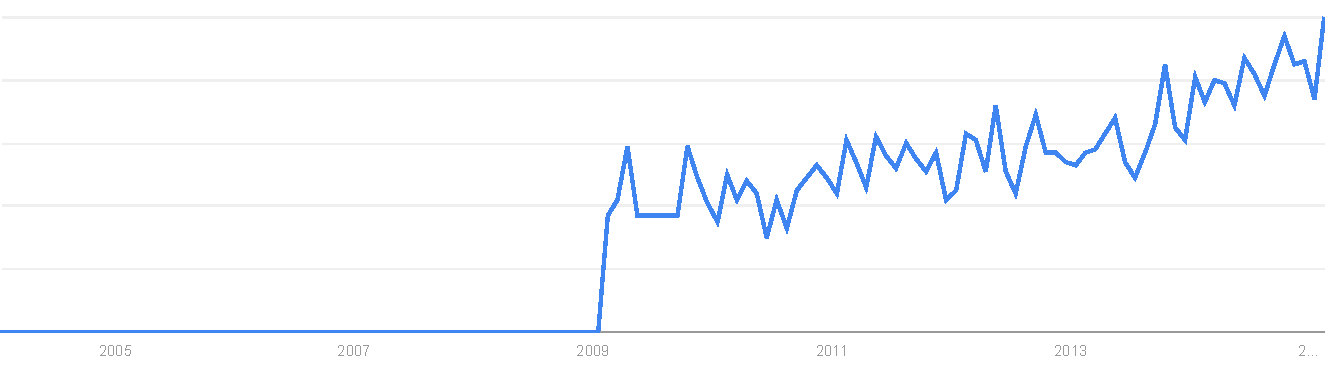
\includegraphics[width=\textwidth]{figure/technicalDebt.pdf}
    \caption{Popularity of \textit{Technical Debt} in Google over time.}
    \label{fig:technical_debt_trend}
\end{figure}

The report is articulated as follows. Section \ref{related_work} presents the relevant related work available to date on the topic. Section 3 contains an accurate description of the research methodology followed. Section 4 illustrates the data that has been gathered which is subsequently analyzed and discussed in Section 5. Section 6 contains the conclusions and possible future works on the topic. Finally, Section 7 will discuss Threats to Validity and all the steps taken to lessen them.
